%!TEX encoding=UTF-8
\documentclass[ 4paper,11pt,openany]{book}
\usepackage[T1]{fontenc}
\usepackage[english,italian]{babel}
\usepackage{graphicx}
\usepackage[margin=1in]{geometry}
\usepackage{listings}
\usepackage{xcolor}

\title{Progetto Lavoratori Stagionali}
\author{Christian Farina\\Stefano Zenaro}
\date{Anno 2021/2022}

\begin{document}
\frontmatter
\maketitle
\tableofcontents 

\mainmatter
\chapter{Introduzione}
\section{Consegna}
Si vuole progettare un sistema informatico di una agenzia che fornisce servizi di supporto alla ricerca di lavoro stagionale. I lavoratori interessati possono iscriversi al servizio, rivolgendosi agli sportelli dell’agenzia. Il sistema deve permettere la gestione delle anagrafiche e la ricerca di lavoratori
stagionali, nei settori dell’agricoltura e del turismo. 

I responsabili del servizio, dipendenti dell’agenzia, inseriscono i dati dei lavoratori. 
Per ogni lavoratore vengono memorizzati i dati anagrafici (nome, cognome, luogo e data di nascita, nazionalità), indirizzo, recapito telefonico personale (se presente), email, le eventuali
specializzazioni/esperienze precedenti (bagnino, barman, istruttore di nuoto, viticultore,floricultore), lingue parlate, il tipo di patente di guida e se automunito. Sono inoltre memorizzati i periodi e le zone (comuni), per i quali il lavoratore è disponibile. Di ogni lavoratore si memorizzano anche le informazioni di almeno una persona da avvisare in caso di urgenza: nome, cognome, telefono, indirizzo email. 

I dipendenti dell’agenzia devono autenticarsi per poter accedere al sistema e inserire i dati dei lavoratori. Il sistema permette ai dipendenti dell’agenzia di aggiornare le anagrafiche con tutti ilavori che i lavoratori stagionali hanno svolto negli ultimi 5 anni. 
Per ogni lavoro svolto vanno registrati: periodo, nome dell’azienda, mansioni svolte, luogo di lavoro, retribuzione lorda giornaliera. Per i dipendenti dell’agenzia si memorizzano i dati anagrafici, l’indirizzo email, il telefono e le credenziali di accesso (login e password).

Una volta registrate le informazioni sui lavoratori, il personale dell’agenzia può effettuare ricerche rispetto a possibili profili richiesti.
In particolare, il sistema deve permettere ai dipendenti di effettuare ricerche per lavoratore, per lingue parlate, periodo di disponibilità, mansioni indicate, luogo di residenza, disponibilità di auto/patente di guida. Il sistema deve permettere di effettuare ricerche complesse, attraverso la specifica di differenti condizioni di ricerca (sia in AND che in OR).
\section{Metodologia di lavoro adottata}
La metodologia di lavoro da noi adottata si avvicina molto al modello plan driven, infatti tutte le attività del processo sono state pianificate in anticipo secondo un modello a cascata che prevedeva l'analisi iniziale dei requisiti, la progettazione del software da un punto di vista ad alto livello, la realizzazione dello stesso tramite il linguaggio di programmazione Java e una fase finale di test per verificare la corretta funzionalità del prodotto finale.
Questa metodologia di sviluppo è stata usata maggiormente nella parte di sviluppo dell'interfaccia grafica e di tutta la parte relativa ai controlli gestiti da quest'ultima, la parte del progetto riguardante la gestione dei dati (memorizzazione lettura ecc.) è stata ideata seguendo una strategia più vicina al metodo agile con pianificazione incrementale; man mano che venivano aggiunte nuove funzionalità, si procedeva con una fase di test e validazione. La parte grafica del progetto è stata invece testata a parte, solo alla conclusione del processo sono stati eseguiti test che coinvolgevano entrambe le parti dell'applicazione. Il lavoro è stato gestito con la metodologia scrum, i compiti da eseguire erano principalmente suddivisi in compiti riguardanti il front end e compiti riguardanti il back end. 
Il lavoro e la condivisione del progetto sono stati gestiti grazie al software di controllo di versione git e GitHub che permette di lavorare in gruppo in maniera efficiente anche modificando il progetto in maniera asincrona (su branch differenti) per poi combinare le diverse modifiche (merge) fatte in un secondo momento, per questo non è stato necessario incontrarsi spesso per decidere come procedere col lavoro.  Di seguito è riportato un breve schema che riassume la divisione dei lavori, a sinistra il nome e a destra la lista dei compiti svolti.\\ \\
\begin{tabular}{|c|c|c|c|c|}
\hline
\textbf{Christian Farina} & Finestre & Controlli delle finestre & Validazione dell'inserimento & Test della view\\
\hline
\textbf{Stefano Zenaro} & Gestione dati & Validazione dei dati & Salvataggio su file & Test del model\\
\hline
\end{tabular}

\chapter{Struttura del progetto}
In questo capitolo sarà descritta la struttura generale del progetto e come esso si presenta all'utente finale. Verranno poi mostrati alcuni esempi di casi d'uso principali con relativi diagrammi di sequenza, per concludere sarà mostrato un diagramma riassuntivo delle attività generali.

\section{Casi d'uso principali}
Il diagramma dei casi d'uso raffigurato qui sotto mostra i modi principali per utilizzare questa applicazione, di seguito sono riportati i singoli casi d'uso descritti più nel dettaglio.\\
\advance\leftskip-0.5cm
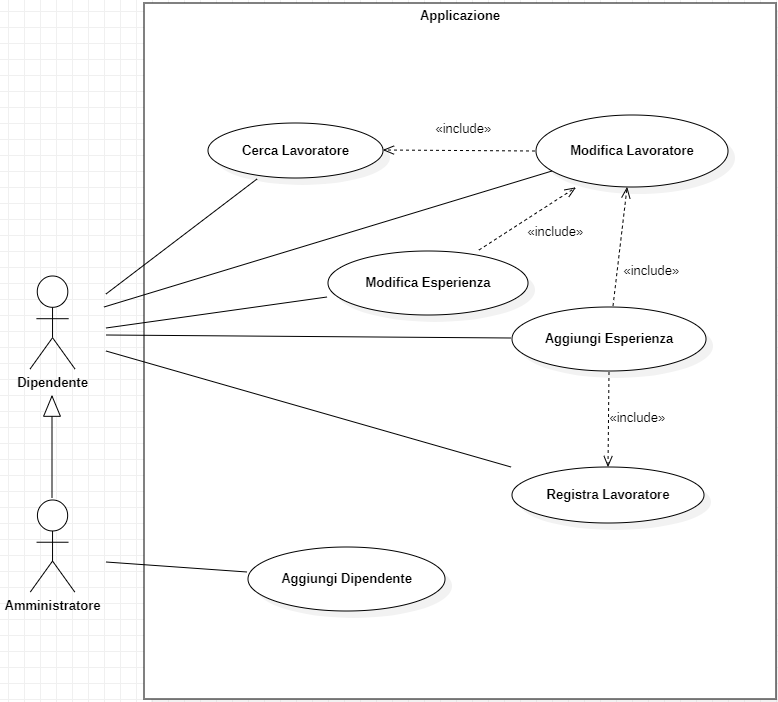
\includegraphics[width=180mm]{casi.png}

\subsection{Registrazione di un lavoratore con rispettiva esperienza lavorativa}
\textbf{Precondizioni}: l'utente deve essere autenticato\\
\textbf{Attore}: Dipendente (può essere anche l'amministratore)\\
\textbf{Passi}:
\begin{enumerate}
\item Il dipendente registra un nuovo lavoratore
\item Il dipendente cerca il lavoratore appena creato, apre la sua pagina di modifica 
\item Il dipendente aggiunge una nuova esperienza lavorativa tramite la pagina di modifica del lavoratore
\end{enumerate}
\textbf{Postcondizioni}: un nuovo lavoratore con un'esperienza lavorativa è stato inserito\\

\subsection{Modifica di un lavoratore}
\textbf{Precondizioni}: l'utente deve essere autenticato\\
\textbf{Attore}: Dipendente (può essere anche l'amministratore)\\
\textbf{Passi}:
\begin{enumerate}
\item Il dipendente cerca il lavoratore tramite la pagina di ricerca
\item Il dipendente apre la scheda del lavoratore cliccando sulla tabella 
\item Il dipendente modifica il lavoratore
\item Il dipendente salva le modifiche
\end{enumerate}
\textbf{Postcondizioni}: un lavoratore è stato modificato\\

\subsection{Modifica di un'esperienza lavorativa}
\textbf{Precondizioni}: l'utente deve essere autenticato\\
\textbf{Attore}: Dipendente (può essere anche l'amministratore)\\
\textbf{Passi}:
\begin{enumerate}
\item Il dipendente cerca il lavoratore
\item Il dipendente apre la scheda del lavoratore cliccando sulla tabella
\item Il dipendente apre la scheda con l'elenco delle esperienze lavorative
\item Il dipendente seleziona l'esperienza interessata e la modifica
\item Il dipendente salva le modifiche
\end{enumerate}
\textbf{Postcondizioni}: un'esperienza lavorativa è stata modificata\\

\subsection{Registrazione di un nuovo dipendente}
\textbf{Precondizioni}: l'utente deve essere autenticato come amministratore\\
\textbf{Attore}: Amministratore\\
\textbf{Passi}:
\begin{enumerate}
\item L'amministratore apre la finestra per aggiungere i dipendenti 
\item Registra un nuovo dipendente
\end{enumerate}
\textbf{Postcondizioni}: un nuovo dipendente è stato inserito\\

\section{Diagrammi di sequenza dei casi d'uso}
Qui di sotto sono raffigurati i diagrammi di sequenza dei casi d'uso spiegati in precedenza, è stato scelto di dividere il diagramma in due parti a seconda dell'attore interessato al fine di garantire una maggiore leggibilità. La prima immagine raffigura i passaggi per la creazione e modifica di un lavoratore, la seconda i passi per creare un nuovo dipendente.
\subsection{Creazione e modifica di un lavoratore}
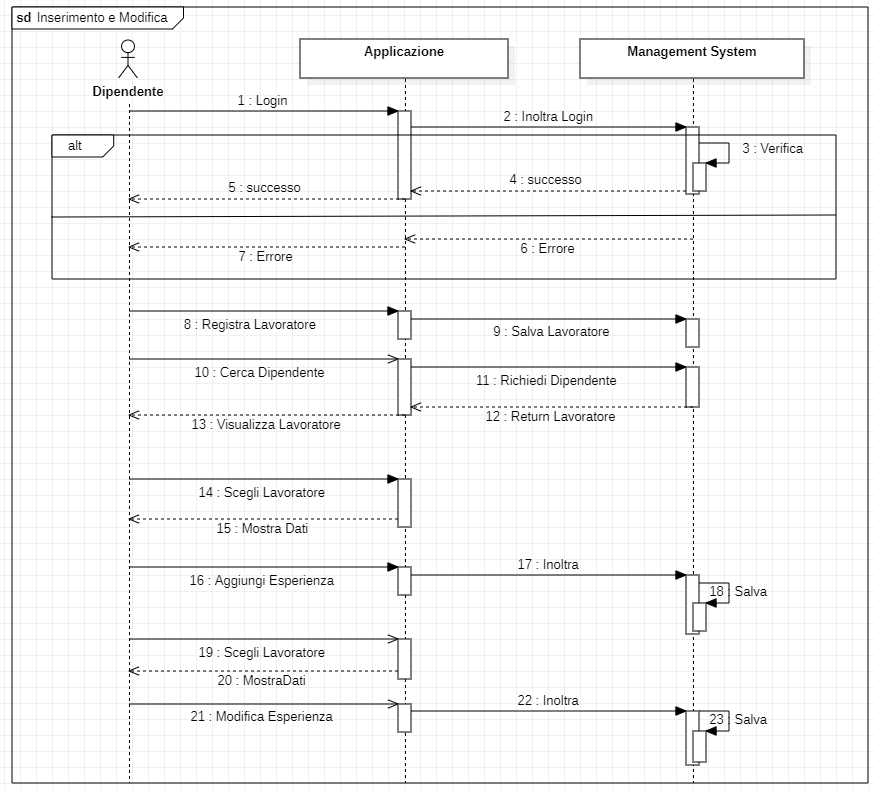
\includegraphics[width=180mm]{seq.png}
\subsection{Creazione di un dipendente}
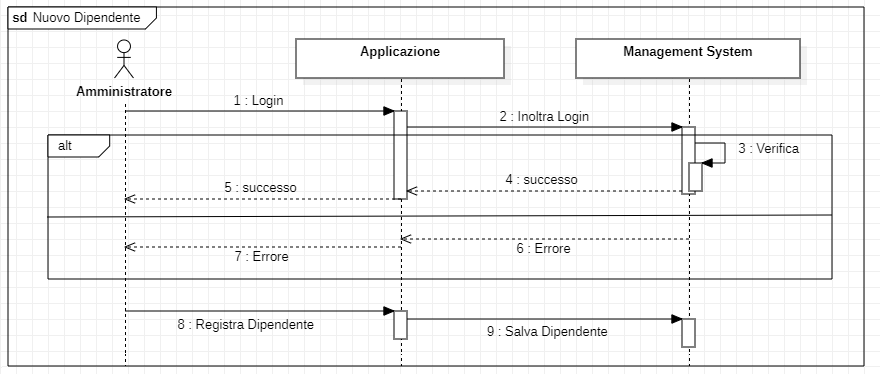
\includegraphics[width=180mm]{seq2.png}
\section{Diagramma delle attività}
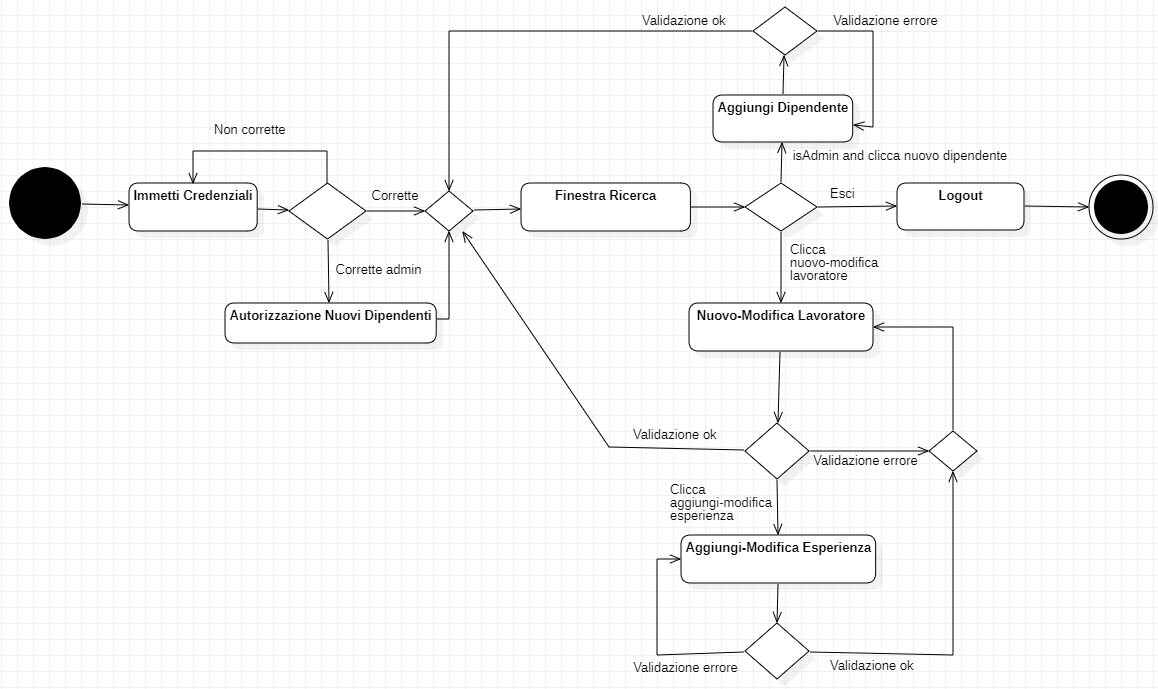
\includegraphics[width=185mm]{attivita.png}

\chapter{Implementazione}
In questo capitolo verrà trattato tutto ciò che è strettamente legato ai metodi implementativi usati per la realizzazione di questa applicazione. Verranno inoltre descritti i pattern architetturali e di design utilizzati.
\section{Classi implementate}
Di seguito è riportato un elenco delle classi suddivise per tipologia, seguirà poi un diagramma delle classi UML dove saranno rappresentate solo le classi utili per far comprendere la struttura generale del progetto, saranno omesse le variabili utilizzate e i metodi, per garantire una migliore leggibilità.\\\\
\textbf{Classi per la gestione dei dati}
\begin{itemize}
\item ManagementSystem
\item ManagementSystemResponse
\item ManagementSystemStatus (enumerazione)
\end{itemize}
\textbf{Classi per la grafica}
\begin{itemize}
\item FinestraContatto
\item FinestraDipendente
\item FinestraEsperienzaLavorativa
\item FinestraLavoratore
\item FinestraLogin 
\item FinestraModificaEsperienze
\item FinestraRicerca
\item FinestraVisualizzaContatti
\end{itemize}
\textbf{Classi che rappresentano i dati da memorizzare}
\begin{itemize}
\item Admin
\item Comune (enumerazione)
\item Dipendente
\item EsperienzaLavorativa
\item Lavoratore
\item Lingua (enumerazione)
\item Patente (enumerazione)
\item PeriodoDisponibilita
\item Persona
\item PersonaInterface
\item RecapitoUrgenze
\end{itemize}

\section{Diagramma delle classi}
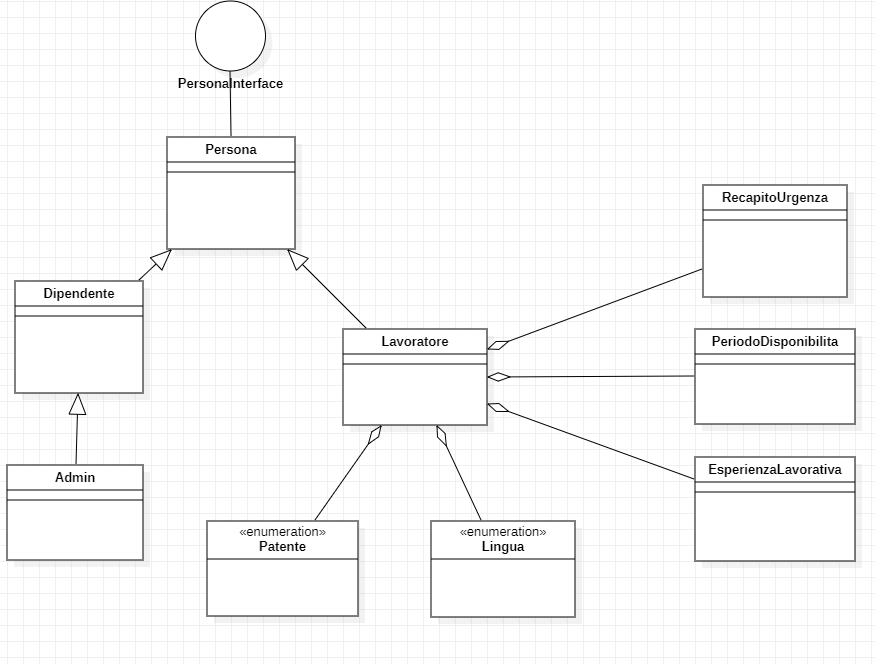
\includegraphics[width=185mm]{classi.png}
Nota: le parti di rappresentazione delle classi riguardanti l'interfaccia grafica e il Management system sono state omesse poichè non fondamentali per capire l'organizzazione dell'applicazione.
\section{Diagrammi di sequenza del software}
In questa sezione verranno mostrati i diagrammi di sequenza visti in precedenza, dal punto di vista del software progettato. Sono state omesse le parti di registrazione dell'utente per garantire una migliore leggibilità. Le linee di vita sono quelle dei vari componenti che costituiscono l'applicazione, saranno quindi mostrate più in dettaglio le interazioni delle singole parti.
\subsection{Creazione e modifica di un lavoratore}
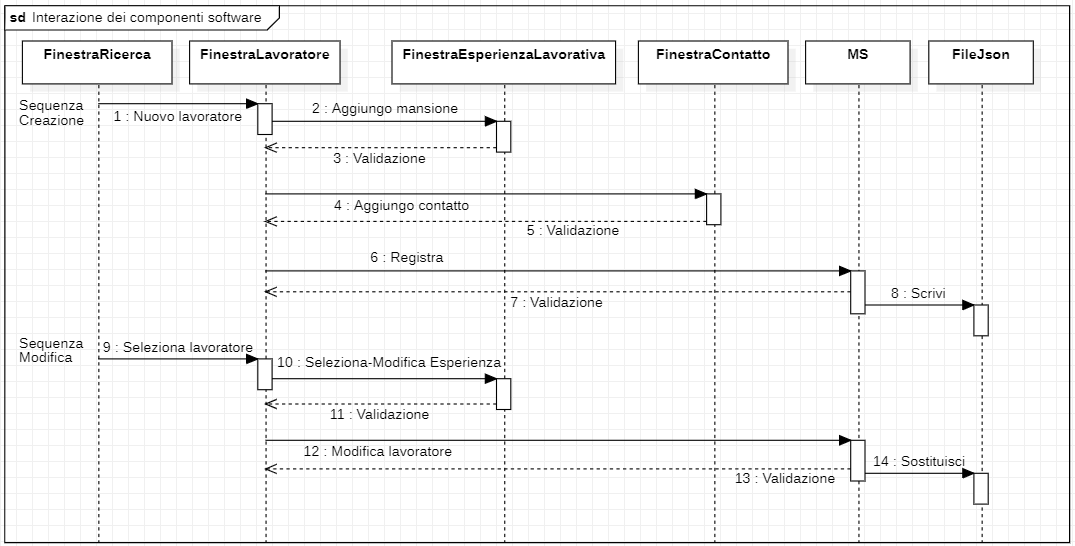
\includegraphics[width=180mm]{softwareseq.png}
\subsection{Creazione di un dipendente}
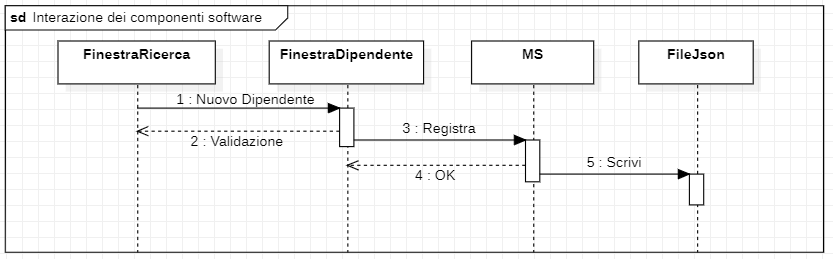
\includegraphics[width=180mm]{softwareseq2.png}

\section{Pattern architetturale: MVC}
Per scrivere l'applicazione si e' deciso di implementare il pattern architetturale Model~View~Controller (MVC).
E' stato utilizzato il pattern MVC perche' permettere di separare le responsabilita' dell'applicazione in tre parti:
\begin{itemize}
    \item Model: il modello e' la logica interna della applicazione. Questa parte gestisce il login, l'inserimento, la ricerca e l'eliminazione dei dati, la lettura e la scrittura dei dati in modo permanente su disco.
    \item View: la vista e' la parte grafica che gestisce cio' che e' visibile dall'utente. Attraverso FXML e' possibile rappresentare pulsanti, tabelle e label.
    \item Controller: il controllore gestisce l'interazione dell'utente con l'interfaccia grafica permettendo la comunicazione tra la vista e il modello.
\end{itemize}
\begin{center}
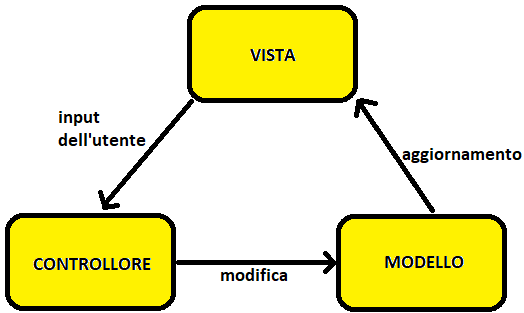
\includegraphics{mvc.png}
\end{center}

\section{Pattern di design: Singleton}
Per gestire creazione, elaborazione ed eliminazione dei dati e' stata creata una classe chiamata ManagementSystem che e' implementata seguendo il pattern Singleton.
Il pattern Singleton garantisce che all'interno della applicazione venga creata una sola istanza di questa classe.

Quando la classe viene istanziata viene eseguita la lettura dei file JSON e ad ogni inserimento o modifica dei dati questi vengono scritti su file.
Il vantaggio del pattern singleton applicato a questo approccio è che permette di poter richiedere facilmente l'istanza all'interno di un qualsiasi controller garantendo che non sarà mai possibile avere stati indeterminati o multipli del sistema: è sempre presente un unico stato che evolve nel tempo con la sua copia memorizzata su disco in formato JSON.

Il motivo per cui è stato deciso di utilizzare questo tipo di pattern è la possibilità di trattare il ManagementSystem come una vera e propria base di dati, tutte le volte che viene richiesto un servizio al model, quest'ultimo viene infatti "interrogato". Possiamo quindi vedere i metodi del MS come una sorta di query che all'occorrenza forniscono i dati richiesti.

Grazie a tale pattern è stato inoltre possibile implementare la visualizzazione in forma tabulare dei lavoratori e il rispettivo sistema di ricerca, tramite interfaccia grafica è infatti possibile eseguire ricerche in and e or gestite quasi totalmente da due metodi del MS.

\section{Pattern di design: DAO}
La classe ManagementSystem, oltre ad essere stata implementata seguendo il pattern Singleton, segue anche il pattern Data Access Object pattern: in questo pattern solo alcuni oggetti possono leggere e scrivere dati su file (o su database) e il loro compito e' fornire un'interfaccia per interagire con i dati.

\chapter{Test}
In questo capitolo verranno spiegate le principali attività di test che sono state effettuate, sarà fornito anche un esempio pratico di una parte di codice utilizzata per testare l'applicazione. In conclusione si descriverà brevemente anche la prova con utente generico e come è risultata utile al miglioramento del software. 
\section{Test del software}
Per testare il sistema sono stati implementati degli unit test per verificare il buon funzionamento di ogni metodo implementato nel modello. Le varie prove sono state effettuate in concomitanza con lo sviluppo del progetto, in particolare è stato testato ogni metodo del ManagementSystem con il framework JUnit5 che permette di creare metodi che si dedicano esclusivamente alle operazioni di testing delle applicazioni.  Per la generazione di dati casuali è stata usata la libreria Faker, di seguito alcuni esempi:\\\\
\textbf{Generazione casuale di un lavoratore}
\begin{lstlisting}[basicstyle=\small,xleftmargin=-0.5cm]
private Lavoratore generateLavoratore(boolean validData){
	// crea data attuale e sottraici 20 anni
        Date twentyYearsAgo = new Date();
        twentyYearsAgo.setYear(twentyYearsAgo.getYear()-20);

        Lavoratore lavoratore;

        if (validData) {
            lavoratore = Lavoratore.of(
                faker.name().firstName(),
                faker.name().lastName(),
                faker.address().streetAddress(),
                faker.date().past(365 * 10, TimeUnit.DAYS, twentyYearsAgo).toInstant().
		   atZone(ZoneId.systemDefault()).toLocalDate(),
                faker.address().country(),
                faker.internet().emailAddress(),
                generateTelephoneNumber(),
                faker.address().streetAddress(),
                List.of(),
                List.of(),
                List.of(),
                false,
                List.of(),
                List.of(
                    RecapitoUrgenza.of(
                        faker.name().firstName(),
                        faker.name().lastName(),
                        generateTelephoneNumber(),
                        faker.internet().emailAddress()
                    )
                ),
                generateCodiceFiscale()
            );
        }
        else{
            lavoratore = Lavoratore.of(
                faker.name().firstName(),
                faker.name().lastName(),
                faker.address().streetAddress(),
                faker.date().future(10, TimeUnit.DAYS).toInstant().
		   atZone(ZoneId.systemDefault()).toLocalDate(),
                faker.address().country(),
                faker.internet().emailAddress(),
                generateTelephoneNumber(),
                faker.address().streetAddress(),
                List.of(),
                List.of(),
                List.of(),
                false,
                List.of(),
                List.of(),
                generateCodiceFiscale()
            );
        }

        return lavoratore;
}
\end{lstlisting}
\textbf{Generazione casuale di un'esperienza lavorativa}
\begin{lstlisting}[basicstyle=\small,xleftmargin=-0.5cm]
private EsperienzaLavorativa generateEsperienzaLavorativa(boolean validData){
       HashSet<String> mansioniSvolte = new HashSet<>();
       for (int i = 0; i < faker.number().numberBetween(1, 10); i++)
           mansioniSvolte.add(faker.job().title());

        EsperienzaLavorativa esperienzaLavorativa;
        if (validData){
            esperienzaLavorativa = EsperienzaLavorativa.of(
                dateToLocalDate(faker.date().between(new Date(2000, Calendar.JANUARY, 1),
		   new Date(2000, Calendar.DECEMBER, 31))),
                dateToLocalDate(faker.date().between(new Date(2001, Calendar.JANUARY, 1),
		   new Date(2001, Calendar.DECEMBER, 31))),
                faker.company().name(),
                mansioniSvolte,
                faker.address().streetAddress(),
                faker.number().numberBetween(50, 200)
            );
        }
        else{
            esperienzaLavorativa = EsperienzaLavorativa.of(
                dateToLocalDate(faker.date().between(new Date(2000, Calendar.JANUARY, 1),
		   new Date(2000, Calendar.DECEMBER, 31))),
                dateToLocalDate(faker.date().between(new Date(2001, Calendar.JANUARY, 1),
		   new Date(2001, Calendar.DECEMBER, 31))),
                "",
                mansioniSvolte,
                faker.address().streetAddress(),
                faker.number().numberBetween(50, 200)
            );
        }
	return esperienzaLavorativa;
}
\end{lstlisting}
\textbf{Generazione casuale di un dipendente}
\begin{lstlisting}[basicstyle=\small,xleftmargin=-0.5cm,]
private Dipendente generateDipendente(boolean validData){
        // crea data attuale e sottraici 20 anni
        Date twentyYearsAgo = new Date();
        twentyYearsAgo.setYear(twentyYearsAgo.getYear()-20);

        Dipendente dipendente;
        String nome = faker.name().firstName();
        String cognome = faker.name().lastName();
        String username = nome.charAt(0) + cognome;
        String email = username + "@" + faker.internet().domainName() + ".com";

        if (validData) {
            dipendente = Dipendente.of(
                nome,
                cognome,
                faker.address().streetAddress(),
                faker.date().past(365 * 10, TimeUnit.DAYS, twentyYearsAgo).toInstant().
		   atZone(ZoneId.systemDefault()).toLocalDate(),
                faker.address().country(),
                email,
                generateTelephoneNumber(),
                username,
                generateStrongPassword(),
                generateCodiceFiscale()
            );
        }
        else{
            dipendente = Dipendente.of(
                nome,
                cognome,
                faker.address().streetAddress(),
                faker.date().future(10, TimeUnit.DAYS).toInstant().
		   atZone(ZoneId.systemDefault()).toLocalDate(),
                faker.address().country(),
                email,
                generateTelephoneNumber(),
                username,
                "pwdinsicura",
                generateCodiceFiscale()
            );
        }
	return dipendente;
}
\end{lstlisting}
\textbf{Generazione casuale di un amministratore}
\begin{lstlisting}[basicstyle=\small,xleftmargin=-0.5cm]
private Admin generateAdmin(boolean validData){
        // crea data attuale e sottraici 20 anni
        Date twentyYearsAgo = new Date();
        twentyYearsAgo.setYear(twentyYearsAgo.getYear()-20);

        Admin admin;
        String nome = faker.name().firstName();
        String cognome = faker.name().lastName();
        String username = nome.charAt(0) + cognome;
        String email = username + "@" + faker.internet().domainName() + ".com";

        if (validData){
            admin = Admin.of(
                nome,
                cognome,
                faker.address().streetAddress(),
                faker.date().past(365*10, TimeUnit.DAYS, twentyYearsAgo).toInstant().
		   atZone(ZoneId.systemDefault()).toLocalDate(),
                faker.address().country(),
                email,
                generateTelephoneNumber(),
                username,
                generateStrongPassword(),
                generateCodiceFiscale()
            );
        }
        else{
            admin = Admin.of(
                nome,
                cognome,
                faker.address().streetAddress(),
                faker.date().future(10, TimeUnit.DAYS).toInstant().
		   atZone(ZoneId.systemDefault()).toLocalDate(),
                faker.address().country(),
                email,
                generateTelephoneNumber(),
                username,
                "pwdinsicura",
                generateCodiceFiscale()
            );
        }
        return admin;
}
\end{lstlisting}
\textbf{Test del login e logout}
\begin{lstlisting}[basicstyle=\small,xleftmargin=-0.5cm]
void testLoginAndLogout() throws IOException, URISyntaxException {
        ManagementSystem ms = ManagementSystem.getInstance(resourcePath);

        assertNull(ms.getLoggedInUser());

        assertFalse(ms.logout());

        assertThrows(IllegalArgumentException.class, () -> ms.login(null, null));

        assertFalse(ms.login("", ""));
        assertNull(ms.getLoggedInUser());

        assertFalse(ms.login(defaultAdminUsername, ""));
        assertNull(ms.getLoggedInUser());

        assertTrue(ms.login(defaultAdminUsername, defaultAdminPassword));
        assertNotNull(ms.getLoggedInUser());

        assertTrue(ms.logout());
        assertNull(ms.getLoggedInUser());
}
\end{lstlisting}
\textbf{Test per le ricerca dei lavoratori}
\begin{lstlisting}[basicstyle=\small,xleftmargin=-0.5cm]
    void searchLavoratoreAnd() throws IOException, URISyntaxException {
        ManagementSystem ms = ManagementSystem.getInstance(resourcePath + "/search_tests");

        ms.login(defaultAdminUsername, defaultAdminPassword);

        // non specificare nessun filtro: mi aspetto di restituire tutti i lavoratori
        assertEquals(
        new TreeSet<>(ms.getLavoratori()),
        new TreeSet<>(ms.selectLavoratoriAnd(null,null,null,null,null,null,null,null))
        );

        // specifica il nome: dovrebbero esserci solo i lavoratori con questo nome
        List<Lavoratore> lavoratoriVincent = new ArrayList<>(
        ms.selectLavoratoriAnd("Vincent",null,null,null,null,null,null,null)
        );

        for (Lavoratore lavoratore: lavoratoriVincent){
            assertEquals("Vincent", lavoratore.getNome());
        }
}
\end{lstlisting}

Per tutta la parte relativa al test dell'interfaccia grafica sono state eseguite numerose prove manuali che hanno portato ad un miglioramento dell'interfaccia grafica e specialmente ad una maggiore attenzione nei controlli dei dati inseriti tramite TextField. Tali controlli sono stati gestiti a livello del controller poichè non correlati alla validazione dell'input.

\section{Test con utente generico}
Il software è stato presentato ad utenti esterni non a conoscenza della struttura implementativa dell'applicazione, non è stata fornita loro alcun tipo di guida di modo da poter verificare, oltre che la corretta esecuzione del programma, anche l'intuitività dell'interfaccia grafica. Per quanto riguarda la parte funzionale, non sono stati riscontrati problemi rilevanti, è però stato necessario rendere la view del progetto più chiara ed esaustiva, poichè alcune etichette poste sui pulsanti traevano in inganno l'utente inducendolo a pensare ad un'errata funzione che il pulsante avrebbe dovuto eseguire. 

Grazie a questo tipo di test abbiamo inoltre compreso come rendere il sistema più "tollerante" agli inserimenti errati degli utenti permettendo di digitare gli spazi in alcune TextField che mandavano il programma in errore se l'input non era inserito correttamente. Dopo queste correzioni è stata riproposta la possibilità all'utente generico di riutilizzare e quindi rivalutare l'applicazione, nella seconda fase di test il tempo di utilizzo da parte di quest'ultimo si è ridotto notevolmente testimoniando il fatto di un miglioramento della struttura grafica.

\end {document}
